\section{Type structure}
\label{sec:type-structure}

At its core, Roslyn creates tree representations from any given piece of code. Whether this concerns a single statement or an entire class doesn't matter -- in the end, everything is reduced to a tree data structure. We can distinguish 2 different kinds of elements that make up the tree and a 3rd element that augments additional information.

\subsection{Syntax Tree}
\label{sec:syntax-tree}

The syntax tree in itself is the starting point from which a lot of aspects start or end: in a CodeFix you can end up replacing the original tree with the modified one while it might as well be the starting point with which you interpret plain text as something you can inspect.

Creating a syntax tree can be as easy as parsing plain text:

\lstset{style=csharp, caption={}}
\begin{lstlisting}
var tree = CSharpSyntaxTree.ParseText(@"
public class Sample
{
}");
\end{lstlisting}

which will result in the tree as shown in figure \ref{fig:tree-structure-class-definition}

\begin{figure}[h]
\centering
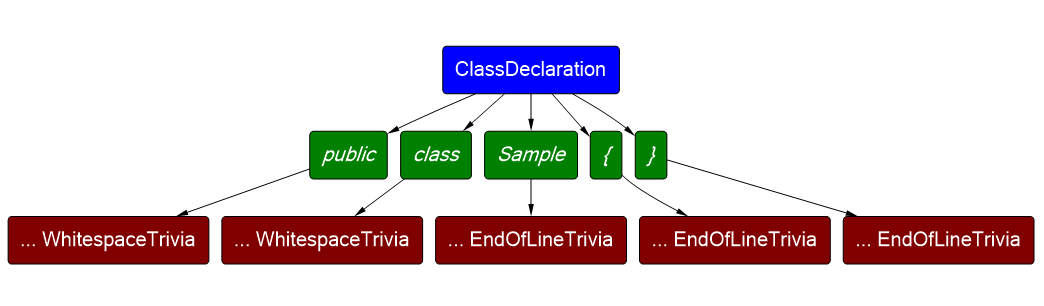
\includegraphics[scale=0.50]{tree-structure-class-definition}
\caption{Syntax tree representation of a class definition}
\label{fig:tree-structure-class-definition}
\end{figure}

A syntax tree represents at the highest level a single top-level type (class or struct) with all its containing members -- fields, methods and nested types. Multiple syntax trees can be grouped in a compilation. It is however not a requirement to represent a type when parsing a syntax tree: any kind of statement or expression can be parsed and represented in a syntax tree. In the end, every syntax node represents a tree of itself. This idea of trees comprised of other trees is what enables interesting performance optimizations (more on that later). 

Syntax trees have a few very important properties:

\begin{itemize}
	\item Full fidelity -- The guarantee that every character, whitespace, comment, line ending, etc from the source code is represented in the syntax tree.
	\item Round-trippable -- Following from the above: translating the source code to a syntax tree and back results in exactly the same code.
	\item Code as written, not as executed -- When you use the \verb|async| and \verb|await| keywords it will represent these keywords in the syntax tree and not the state machine that the compiler generates from it.
	\item Immutable -- Every syntax tree is immutable. This allows for thread-safe operations since everything handles its own "copy" of the syntax tree anyway.
\end{itemize}

\subsection{Syntax Node}
\label{sec:syntax-node}

A syntax node is an element of the tree that is always the parent to other nodes or to tokens (also known as 'non-terminal') and represents an expression or a statement. 

Syntax nodes are defined in the Syntax.xml\footnote{https://github.com/dotnet/roslyn/blob/master/src/Compilers/CSharp/Portable/Syntax/Syntax.xml} file which generates classes that represent the relationship between all kinds of syntax nodes. 

[More info on syntax.xml]

\subsection{Syntax Token}
\label{sec:syntax-token}

Syntax tokens are what make up the individual, small pieces of the code. Whereas syntax nodes mainly represent the syntactic constructs of the language, syntax tokens are the building blocks that these syntactic constructs consist of.
A syntax token can be a keyword, identifier, literal and punctuation and only exists as a leaf in the tree: it will never be the parent of another node or token.

Contrary to syntax nodes, syntax tokens are not represented by separate classes. Instead, a single struct exists which can be differentiated based on its \verb|Kind| property. 

[Look it up][Syntax.xml?]

\subsection{Syntax Trivia}
\label{sec:syntax-trivia}

The last aspect of the tree is the syntax trivia. This is slightly misleading because it's not actually a part of the tree: it is stored as a property on a syntax token. This stems from the idea that syntax tokens could not have child nodes and as such it is implemented by adding it to a token's \verb|LeadingTrivia| and \verb|TrailingTrivia| properties. 

Syntax trivia is the rest of the source code with no actual semantic meaning: comments, whitespace, newlines, etc. Important to note are preprocessing directives: these are also considered trivia.

It is important to represent the trivia inside the syntax tree in order to ensure full-fidelity: if we wouldn't, we would have a differently layed out source code after translating our source to a syntax tree and back.




